\documentclass[border=3pt,tikz]{standalone}
\usepackage{tikz}
\usetikzlibrary{positioning}

\begin{document}
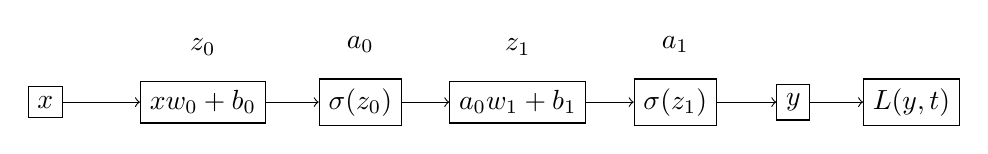
\begin{tikzpicture}
    \node[draw] (x) at (0,0) {$x$};
    \node[draw] (z_0) at (2,0) {$xw_0 + b_0$};
    \node[draw] (a_0) at (4,0) {$\sigma(z_0)$};
    \node[draw] (z_1) at (6,0) {$a_0w_1 + b_1$};
    \node[draw] (a_1) at (8,0) {$\sigma(z_1)$};
    \node[draw] (y) at (9.5,0) {$y$};
    \node[draw] (loss) at (11,0) {$L(y, t)$};
    \draw[->] (x) -- (z_0);
    \draw[->] (z_0) -- (a_0); 
    \draw[->] (a_0) -- (z_1);
    \draw[->] (z_1) -- (a_1);
    \draw[->] (a_1) -- (y);
    \draw[->] (y) -- (loss);
    \node[above=0.2cm of z_0] (z_0) {$z_0$};
    \node[above=0.2cm of a_0] (a_0) {$a_0$};
    \node[above=0.2cm of z_1] (z_1) {$z_1$};
    \node[above=0.2cm of a_1] (a_1) {$a_1$};
\end{tikzpicture}
\end{document}
% how do i draw symbol over the boxes?
